
%%%%%%%%%%%%%%%%%% PREAMBULE %%%%%%%%%%%%%%%%%%

\documentclass[aspectratio=169,utf8]{beamer}
%\documentclass[aspectratio=169,handout]{beamer}

\usetheme{Boadilla}
%\usecolortheme{seahorse}
%\usecolortheme[RGB={245,66,24}]{structure}
\useoutertheme{infolines}

% packages
\usepackage{amsfonts,amsmath,amssymb,amsthm}
\usepackage[utf8]{inputenc}
\usepackage[T1]{fontenc}
\usepackage{lmodern}

\usepackage[francais]{babel}
\usepackage{fancybox}
\usepackage{graphicx}

\usepackage{float}
\usepackage{xfrac}

%\usepackage[usenames, x11names]{xcolor}
\usepackage{pgfplots}
\usepackage{datetime}


% ----------------------------------------------------------------------
% Pour les images
\usepackage{tikz}
\usetikzlibrary{calc,shadows,arrows.meta,patterns,matrix}

\newcommand{\tikzinput}[1]{\input{figures/#1.tikz}}
% --- les figures avec échelle éventuel
\newcommand{\myfigure}[2]{% entrée : échelle, fichier(s) figure à inclure
\begin{center}\small%
\tikzstyle{every picture}=[scale=1.0*#1]% mise en échelle + 0% (automatiquement annulé à la fin du groupe)
#2%
\end{center}}



%-----  Package unités -----
\usepackage{siunitx}
\sisetup{locale = FR,detect-all,per-mode = symbol}

%\usepackage{mathptmx}
%\usepackage{fouriernc}
%\usepackage{newcent}
%\usepackage[mathcal,mathbf]{euler}

%\usepackage{palatino}
%\usepackage{newcent}
% \usepackage[mathcal,mathbf]{euler}



% \usepackage{hyperref}
% \hypersetup{colorlinks=true, linkcolor=blue, urlcolor=blue,
% pdftitle={Exo7 - Exercices de mathématiques}, pdfauthor={Exo7}}


%section
% \usepackage{sectsty}
% \allsectionsfont{\bf}
%\sectionfont{\color{Tomato3}\upshape\selectfont}
%\subsectionfont{\color{Tomato4}\upshape\selectfont}

%----- Ensembles : entiers, reels, complexes -----
\newcommand{\Nn}{\mathbb{N}} \newcommand{\N}{\mathbb{N}}
\newcommand{\Zz}{\mathbb{Z}} \newcommand{\Z}{\mathbb{Z}}
\newcommand{\Qq}{\mathbb{Q}} \newcommand{\Q}{\mathbb{Q}}
\newcommand{\Rr}{\mathbb{R}} \newcommand{\R}{\mathbb{R}}
\newcommand{\Cc}{\mathbb{C}} 
\newcommand{\Kk}{\mathbb{K}} \newcommand{\K}{\mathbb{K}}

%----- Modifications de symboles -----
\renewcommand{\epsilon}{\varepsilon}
\renewcommand{\Re}{\mathop{\text{Re}}\nolimits}
\renewcommand{\Im}{\mathop{\text{Im}}\nolimits}
%\newcommand{\llbracket}{\left[\kern-0.15em\left[}
%\newcommand{\rrbracket}{\right]\kern-0.15em\right]}

\renewcommand{\ge}{\geqslant}
\renewcommand{\geq}{\geqslant}
\renewcommand{\le}{\leqslant}
\renewcommand{\leq}{\leqslant}
\renewcommand{\epsilon}{\varepsilon}

%----- Fonctions usuelles -----
\newcommand{\ch}{\mathop{\text{ch}}\nolimits}
\newcommand{\sh}{\mathop{\text{sh}}\nolimits}
\renewcommand{\tanh}{\mathop{\text{th}}\nolimits}
\newcommand{\cotan}{\mathop{\text{cotan}}\nolimits}
\newcommand{\Arcsin}{\mathop{\text{arcsin}}\nolimits}
\newcommand{\Arccos}{\mathop{\text{arccos}}\nolimits}
\newcommand{\Arctan}{\mathop{\text{arctan}}\nolimits}
\newcommand{\Argsh}{\mathop{\text{argsh}}\nolimits}
\newcommand{\Argch}{\mathop{\text{argch}}\nolimits}
\newcommand{\Argth}{\mathop{\text{argth}}\nolimits}
\newcommand{\pgcd}{\mathop{\text{pgcd}}\nolimits} 


%----- Commandes divers ------
\newcommand{\ii}{\mathrm{i}}
\newcommand{\dd}{\text{d}}
\newcommand{\id}{\mathop{\text{id}}\nolimits}
\newcommand{\Ker}{\mathop{\text{Ker}}\nolimits}
\newcommand{\Card}{\mathop{\text{Card}}\nolimits}
\newcommand{\Vect}{\mathop{\text{Vect}}\nolimits}
\newcommand{\Mat}{\mathop{\text{Mat}}\nolimits}
\newcommand{\rg}{\mathop{\text{rg}}\nolimits}
\newcommand{\tr}{\mathop{\text{tr}}\nolimits}


%----- Structure des exercices ------

\newtheoremstyle{styleexo}% name
{2ex}% Space above
{3ex}% Space below
{}% Body font
{}% Indent amount 1
{\bfseries} % Theorem head font
{}% Punctuation after theorem head
{\newline}% Space after theorem head 2
{}% Theorem head spec (can be left empty, meaning ‘normal’)

%\theoremstyle{styleexo}
\newtheorem{exo}{Exercice}
\newtheorem{ind}{Indications}
\newtheorem{cor}{Correction}


\newcommand{\exercice}[1]{} \newcommand{\finexercice}{}
%\newcommand{\exercice}[1]{{\tiny\texttt{#1}}\vspace{-2ex}} % pour afficher le numero absolu, l'auteur...
\newcommand{\enonce}{\begin{exo}} \newcommand{\finenonce}{\end{exo}}
\newcommand{\indication}{\begin{ind}} \newcommand{\finindication}{\end{ind}}
\newcommand{\correction}{\begin{cor}} \newcommand{\fincorrection}{\end{cor}}

\newcommand{\noindication}{\stepcounter{ind}}
\newcommand{\nocorrection}{\stepcounter{cor}}

\newcommand{\fiche}[1]{} \newcommand{\finfiche}{}
\newcommand{\titre}[1]{\centerline{\large \bf #1}}
\newcommand{\addcommand}[1]{}
\newcommand{\video}[1]{}

% Marge
\newcommand{\mymargin}[1]{\marginpar{{\small #1}}}

\def\noqed{\renewcommand{\qedsymbol}{}}


%----- Presentation ------
\setlength{\parindent}{0cm}

%\newcommand{\ExoSept}{\href{http://exo7.emath.fr}{\textbf{\textsf{Exo7}}}}

\definecolor{myred}{rgb}{0.93,0.26,0}
\definecolor{myorange}{rgb}{0.97,0.58,0}
\definecolor{myyellow}{rgb}{1,0.86,0}

\newcommand{\LogoExoSept}[1]{  % input : echelle
{\usefont{U}{cmss}{bx}{n}
\begin{tikzpicture}[scale=0.1*#1,transform shape]
  \fill[color=myorange] (0,0)--(4,0)--(4,-4)--(0,-4)--cycle;
  \fill[color=myred] (0,0)--(0,3)--(-3,3)--(-3,0)--cycle;
  \fill[color=myyellow] (4,0)--(7,4)--(3,7)--(0,3)--cycle;
  \node[scale=5] at (3.5,3.5) {Exo7};
\end{tikzpicture}}
}


\newcommand{\debutmontitre}{
  \author{} \date{} 
  \thispagestyle{empty}
  \hspace*{-10ex}
  \begin{minipage}{\textwidth}
    \titlepage  
  \vspace*{-2.5cm}
  \begin{center}
    \LogoExoSept{2.5}
  \end{center}
  \end{minipage}

  \vspace*{-0cm}
  
  % Astuce pour que le background ne soit pas discrétisé lors de la conversion pdf -> png
\begin{tikzpicture}
        \fill[opacity=0,green!60!black] (0,0)--++(0,0)--++(0,0)--++(0,0)--cycle; 
\end{tikzpicture}

% toc S'affiche trop tot :
% \tableofcontents[hideallsubsections, pausesections]
}

\newcommand{\finmontitre}{
  \end{frame}
  \setcounter{framenumber}{0}
} % ne marche pas pour une raison obscure

%----- Commandes supplementaires ------

% \usepackage[landscape]{geometry}
% \geometry{top=1cm, bottom=3cm, left=2cm, right=10cm, marginparsep=1cm
% }
% \usepackage[a4paper]{geometry}
% \geometry{top=2cm, bottom=2cm, left=2cm, right=2cm, marginparsep=1cm
% }

%\usepackage{standalone}


% New command Arnaud -- november 2011
\setbeamersize{text margin left=24ex}
% si vous modifier cette valeur il faut aussi
% modifier le decalage du titre pour compenser
% (ex : ici =+10ex, titre =-5ex

\theoremstyle{definition}
%\newtheorem{proposition}{Proposition}
%\newtheorem{exemple}{Exemple}
%\newtheorem{theoreme}{Théorème}
%\newtheorem{lemme}{Lemme}
%\newtheorem{corollaire}{Corollaire}
%\newtheorem*{remarque*}{Remarque}
%\newtheorem*{miniexercice}{Mini-exercices}
%\newtheorem{definition}{Définition}

% Commande tikz
\usetikzlibrary{calc}
\usetikzlibrary{patterns,arrows}
\usetikzlibrary{matrix}
\usetikzlibrary{fadings} 

%definition d'un terme
\newcommand{\defi}[1]{{\color{myorange}\textbf{\emph{#1}}}}
\newcommand{\evidence}[1]{{\color{blue}\textbf{\emph{#1}}}}
\newcommand{\assertion}[1]{\emph{\og#1\fg}}  % pour chapitre logique
%\renewcommand{\contentsname}{Sommaire}
\renewcommand{\contentsname}{}
\setcounter{tocdepth}{2}



%------ Encadrement ------

\usepackage{fancybox}


\newcommand{\mybox}[1]{
\setlength{\fboxsep}{7pt}
\begin{center}
\shadowbox{#1}
\end{center}}

\newcommand{\myboxinline}[1]{
\setlength{\fboxsep}{5pt}
\raisebox{-10pt}{
\shadowbox{#1}
}
}

%--------------- Commande beamer---------------
\newcommand{\beameronly}[1]{#1} % permet de mettre des pause dans beamer pas dans poly


\setbeamertemplate{navigation symbols}{}
\setbeamertemplate{footline}  % tiré du fichier beamerouterinfolines.sty
{
  \leavevmode%
  \hbox{%
  \begin{beamercolorbox}[wd=.333333\paperwidth,ht=2.25ex,dp=1ex,center]{author in head/foot}%
    % \usebeamerfont{author in head/foot}\insertshortauthor%~~(\insertshortinstitute)
    \usebeamerfont{section in head/foot}{\bf\insertshorttitle}
  \end{beamercolorbox}%
  \begin{beamercolorbox}[wd=.333333\paperwidth,ht=2.25ex,dp=1ex,center]{title in head/foot}%
    \usebeamerfont{section in head/foot}{\bf\insertsectionhead}
  \end{beamercolorbox}%
  \begin{beamercolorbox}[wd=.333333\paperwidth,ht=2.25ex,dp=1ex,right]{date in head/foot}%
    % \usebeamerfont{date in head/foot}\insertshortdate{}\hspace*{2em}
    \insertframenumber{} / \inserttotalframenumber\hspace*{2ex} 
  \end{beamercolorbox}}%
  \vskip0pt%
}


\definecolor{mygrey}{rgb}{0.5,0.5,0.5}
\setlength{\parindent}{0cm}
%\DeclareTextFontCommand{\helvetica}{\fontfamily{phv}\selectfont}

% background beamer
\definecolor{couleurhaut}{rgb}{0.85,0.9,1}  % creme
\definecolor{couleurmilieu}{rgb}{1,1,1}  % vert pale
\definecolor{couleurbas}{rgb}{0.85,0.9,1}  % blanc
\setbeamertemplate{background canvas}[vertical shading]%
[top=couleurhaut,middle=couleurmilieu,midpoint=0.4,bottom=couleurbas] 
%[top=fondtitre!05,bottom=fondtitre!60]



\makeatletter
\setbeamertemplate{theorem begin}
{%
  \begin{\inserttheoremblockenv}
  {%
    \inserttheoremheadfont
    \inserttheoremname
    \inserttheoremnumber
    \ifx\inserttheoremaddition\@empty\else\ (\inserttheoremaddition)\fi%
    \inserttheorempunctuation
  }%
}
\setbeamertemplate{theorem end}{\end{\inserttheoremblockenv}}

\newenvironment{theoreme}[1][]{%
   \setbeamercolor{block title}{fg=structure,bg=structure!40}
   \setbeamercolor{block body}{fg=black,bg=structure!10}
   \begin{block}{{\bf Th\'eor\`eme }#1}
}{%
   \end{block}%
}


\newenvironment{proposition}[1][]{%
   \setbeamercolor{block title}{fg=structure,bg=structure!40}
   \setbeamercolor{block body}{fg=black,bg=structure!10}
   \begin{block}{{\bf Proposition }#1}
}{%
   \end{block}%
}

\newenvironment{corollaire}[1][]{%
   \setbeamercolor{block title}{fg=structure,bg=structure!40}
   \setbeamercolor{block body}{fg=black,bg=structure!10}
   \begin{block}{{\bf Corollaire }#1}
}{%
   \end{block}%
}

\newenvironment{mydefinition}[1][]{%
   \setbeamercolor{block title}{fg=structure,bg=structure!40}
   \setbeamercolor{block body}{fg=black,bg=structure!10}
   \begin{block}{{\bf Définition} #1}
}{%
   \end{block}%
}

\newenvironment{lemme}[0]{%
   \setbeamercolor{block title}{fg=structure,bg=structure!40}
   \setbeamercolor{block body}{fg=black,bg=structure!10}
   \begin{block}{\bf Lemme}
}{%
   \end{block}%
}

\newenvironment{remarque}[1][]{%
   \setbeamercolor{block title}{fg=black,bg=structure!20}
   \setbeamercolor{block body}{fg=black,bg=structure!5}
   \begin{block}{Remarque #1}
}{%
   \end{block}%
}


\newenvironment{exemple}[1][]{%
   \setbeamercolor{block title}{fg=black,bg=structure!20}
   \setbeamercolor{block body}{fg=black,bg=structure!5}
   \begin{block}{{\bf Exemple }#1}
}{%
   \end{block}%
}


\newenvironment{miniexercice}[0]{%
   \setbeamercolor{block title}{fg=structure,bg=structure!20}
   \setbeamercolor{block body}{fg=black,bg=structure!5}
   \begin{block}{Mini-exercices}
}{%
   \end{block}%
}


\newenvironment{tp}[0]{%
   \setbeamercolor{block title}{fg=structure,bg=structure!40}
   \setbeamercolor{block body}{fg=black,bg=structure!10}
   \begin{block}{\bf Travaux pratiques}
}{%
   \end{block}%
}
\newenvironment{exercicecours}[1][]{%
   \setbeamercolor{block title}{fg=structure,bg=structure!40}
   \setbeamercolor{block body}{fg=black,bg=structure!10}
   \begin{block}{{\bf Exercice }#1}
}{%
   \end{block}%
}
\newenvironment{algo}[1][]{%
   \setbeamercolor{block title}{fg=structure,bg=structure!40}
   \setbeamercolor{block body}{fg=black,bg=structure!10}
   \begin{block}{{\bf Algorithme}\hfill{\color{gray}\texttt{#1}}}
}{%
   \end{block}%
}


\setbeamertemplate{proof begin}{
   \setbeamercolor{block title}{fg=black,bg=structure!20}
   \setbeamercolor{block body}{fg=black,bg=structure!5}
   \begin{block}{{\footnotesize Démonstration}}
   \footnotesize
   \smallskip}
\setbeamertemplate{proof end}{%
   \end{block}}
\setbeamertemplate{qed symbol}{\openbox}


\makeatother
\usecolortheme[RGB={127,0,0}]{structure}

% Commande spécifique à ce chapitre

\newcommand{\Python}{\texttt{Python}}
\renewcommand{\evidence}[1]{{\color{blue}\textbf{#1}}}

\usepackage{textcomp}

\usepackage{listings}
\lstset{
  upquote=true,
  columns=flexible,
  keepspaces=true,
  basicstyle=\ttfamily,
  commentstyle=\color{gray},
  language=Python,
  showstringspaces=false,
  aboveskip=0em,  
  belowskip=0em,
  escapeinside=||
}

\lstset{
  literate={é}{{\'e}}1
           {è}{{\`e}}1
           {à}{{\`a}}1
}


\newcommand{\codeinline}[1]{\lstinline!#1!}

\definecolor{coul_prive}{rgb}{0.93,0.26,0}
\definecolor{coul_public}{rgb}{0.06,0.63,0}

\newcommand{\prive}[1]{{\bf\color{coul_prive} #1}}
\newcommand{\public}[1]{{\bf\color{coul_public} #1}}

%%%%%%%%%%%%%%%%%%%%%%%%%%%%%%%%%%%%%%%%%%%%%%%%%%%%%%%%%%%%%
%%%%%%%%%%%%%%%%%%%%%%%%%%%%%%%%%%%%%%%%%%%%%%%%%%%%%%%%%%%%%


\begin{document}


\title{{\bf Cryptographie}}
\subtitle{La machine Enigma et les clés secrètes}

\begin{frame}
  
  \debutmontitre

  \pause

{\footnotesize
\hfill
\setbeamercovered{transparent=50}
\begin{minipage}{0.6\textwidth}
  \begin{itemize}
    \item<3-> Un secret parfait
    \item<4-> La machine Enigma
%    \item<5-> Des zéros et des uns
    \item<5-> La ronde des chiffres : DES
  \end{itemize}
\end{minipage}
}

\end{frame}

\setcounter{framenumber}{0}


%%%%%%%%%%%%%%%%%%%%%%%%%%%%%%%%%%%%%%%%%%%%%%%%%%%%%%%%%%%%%%%%
\section{Un secret parfait}

\begin{frame}

\begin{itemize}\setlength{\itemsep}{6pt}
  \item Inconvénient des chiffrements précédents : une même lettre est régulièrement chiffrée de la même façon
\pause  
  \item Une attaque statistique est toujours possible
\pause  
  \item \defi{Chiffrement parfait} : changer la correspondance à chaque lettre
\pause  
  \item Principe 
\pause  
  \begin{itemize}\setlength{\itemsep}{4pt}
    \item deux entiers $m$ et $c$ tels que $m+c=100$. Que vaut $m$ ?
\pause    
    \item c'est bien sûr impossible de répondre
\pause    
    \item $0+100$, $1+99$, $2+98$,...
\pause    
    \item connaissant $c$ alors on trouve $m=100-c$
  \end{itemize}
  
\end{itemize}

\end{frame}


\begin{frame}
\begin{itemize}\setlength{\itemsep}{6pt}
  \item Alice veut envoyer à Bruno le message secret \prive{$M$} 
\centerline{\prive{ATTAQUE \ LE \ CHATEAU}}
\pause

  \item 
  \begin{itemize}\setlength{\itemsep}{4pt}
    \item Alice choisit une clé secrète \prive{$C$}
\pause    
    \item Alice transmet cette clé à Bruno
\pause    
    \item Cette clé a la même longueur que le message
\pause
    \item Elle est composée d'entiers de $0$ à $25$ tirés au hasard
  \end{itemize}
\pause
\smallskip

\centerline{\prive{$C$} = [4, 18, 2, 0, 21, 12, 18, 13, 7, 11, 23, 22, 19, 2, 16, 9]}  

\pause
  \item
  \begin{itemize}\setlength{\itemsep}{4pt}
    \item la première lettre \prive{A} est décalée de $4$ et devient \public{E}
\pause    
    \item le premier \prive{T} est décalé de $18$ lettres et devient \public{L}
 \pause   
    \item le second \prive{T} est décalé de $2$ lettres, il devient \public{V}
 \pause   
    \item le \prive{A} suivant est décalé de $0$ lettre, cela reste \public{A}...
  \end{itemize}

\pause  
  \item Message chiffré \public{$X$}  \\
\centerline{\public{ELVALGW \ YL \ NEWMGQD}}
\end{itemize}


\end{frame}


\begin{frame}

\begin{itemize}
  \item On identifie $A$ avec $0$, $B$ avec $1$, ..., $Z$ avec $25$
\pause  
  \item \! Le message crypté est la somme du message \!\prive{$M$}\! avec la clé secrète\! \prive{$C$}
  \\
  \centerline{\public{$X$} = \prive{$M$} $\oplus$ \prive{$C$}}
 
\pause

\begin{center}
\small
\begin{tabular}{ccccccccc}
&&\prive{A}&\prive{T}&\prive{T}&\prive{A}&\prive{Q}&\prive{U}&\prive{E}\\
&&\prive{0}&\prive{19}&\prive{19}&\prive{0}&\prive{16}&\prive{20}&\prive{4}\\
\pause 
%\multicolumn{7}{l}{$\oplus$}\\
$\oplus$&&\prive{4}&\prive{18}&\prive{2}&\prive{0}&\prive{21}&\prive{12}&\prive{18}\\
\hline
\pause
=&&\public{4}&\public{11}&\public{21}&\public{0}&\public{11}&\public{6}&\public{22}\\
&&\public{E}&\public{L}&\public{V}&\public{A}&\public{L}&\public{G}&\public{W}\\
\end{tabular}
\end{center}


\pause
  \item Bruno reçoit \public{$X$} et connaît \prive{$C$}, donc il effectue \public{$X$} $\ominus$ \prive{$C$} = \prive{$M$}
  
\end{itemize}

\bigskip
\pause

Principes à respecter
\pause
\begin{enumerate}
  \item La longueur de la clé est égale à la longueur du message
\pause 
  \item La clé est choisie au hasard
\pause  
  \item La clé ne sert qu'une seule fois
\end{enumerate}

\bigskip
\pause

Inconvénients
\pause
\begin{itemize}
  \item Clé aussi longue que le message
\pause  
  \item Clé secrète doit être transmise à Bruno
\end{itemize}

\end{frame}


%%%%%%%%%%%%%%%%%%%%%%%%%%%%%%%%%%%%%%%%%%%%%%%%%%%%%%%%%%%%%%%%
\section{La machine Enigma}

\begin{frame}

\begin{minipage}{0.73\textwidth}
\hspace*{-5em}
\begin{itemize}
\uncover<2->{
  \item La machine Enigma est une machine électro-mécanique qui ressemble \\ à une machine à écrire
}
\uncover<3->{
  \item Lorsque qu'une touche est enfoncée, des disques internes sont actionnés et le caractère crypté s'allume
}  
\uncover<4->{
  \item Utilisée pour les communications de l'armée allemande durant la seconde guerre mondiale
}
\uncover<5->{
  \item Les services secrets polonais et britanniques avaient réussi à percer les mystères de ce procédé de chiffrement
}  
\uncover<6->{
  \item Génie d'Alan Turing et l'invention de l’ancêtre de l'ordinateur
}
\end{itemize}  
\end{minipage}
\begin{minipage}{0.2\textwidth}
\hspace*{-4em}
{\centering 
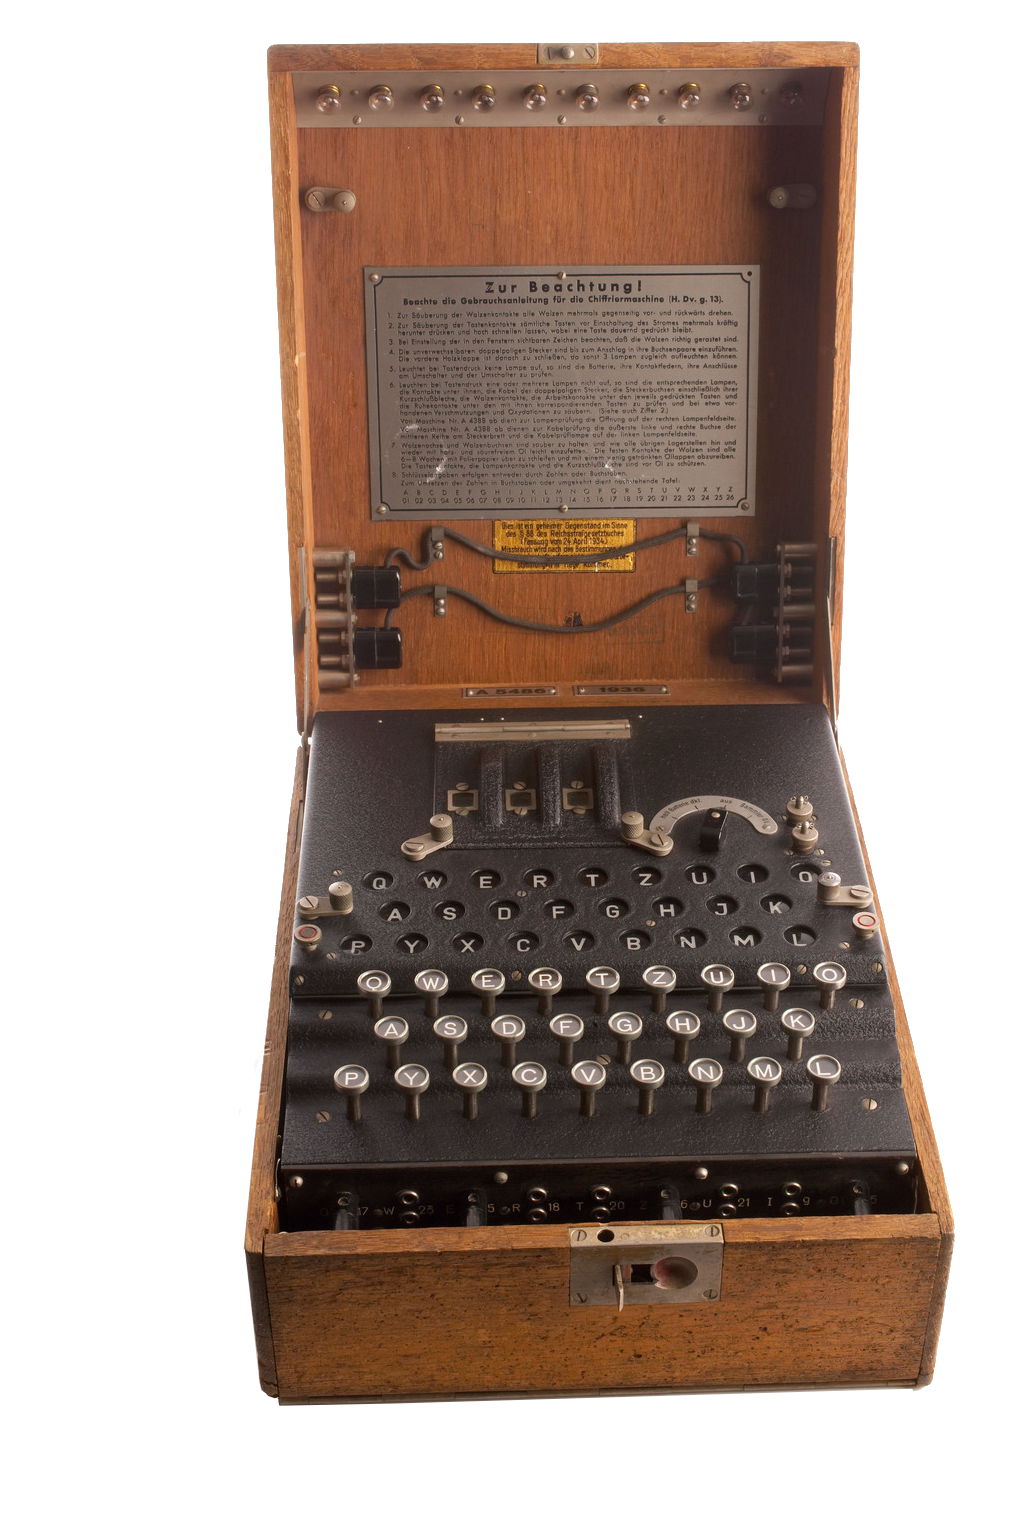
\includegraphics[width=2\textwidth]{figures/Enigma_Machine.png} 
}  
\end{minipage}

\end{frame}


\begin{frame}
Machine Enigma simplifiée à deux anneaux

{\centering 
            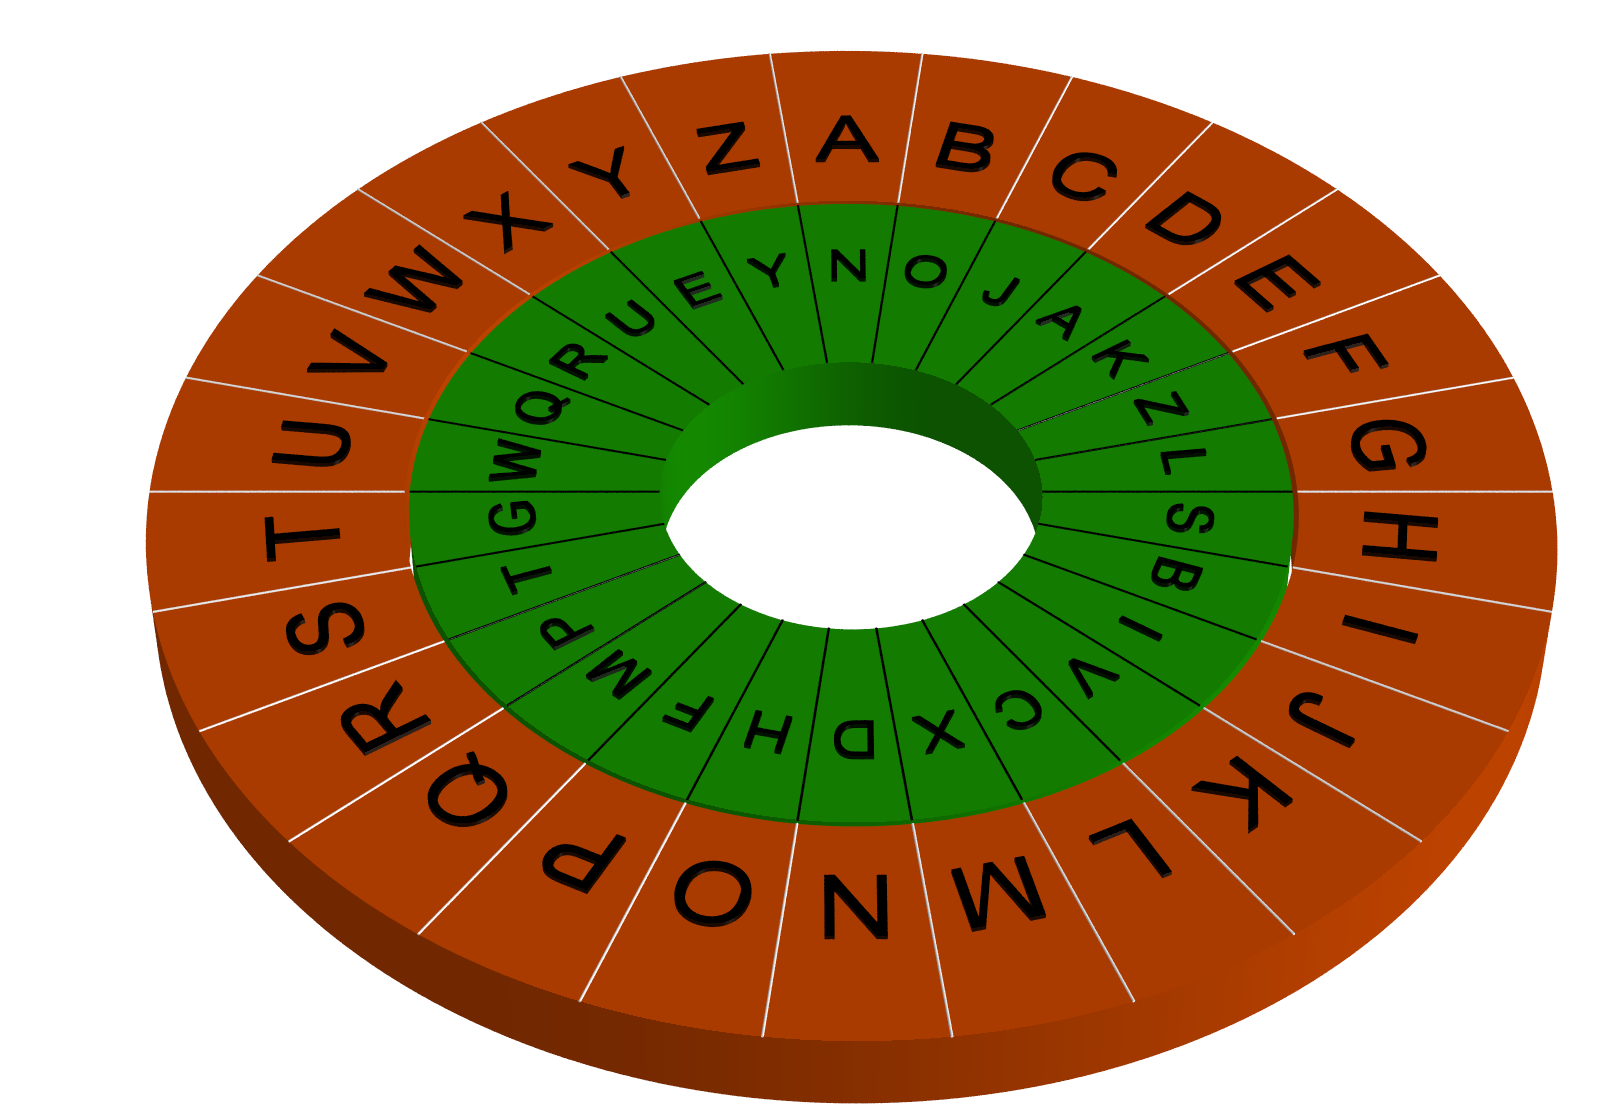
\includegraphics[width=0.4\textwidth]{figures/Enigma_7_bi_unesurune.png} 

}
\pause
\begin{itemize}
  \item Un anneau extérieur fixe contenant l'alphabet \prive{ABCDE...} en clair
\pause  
  \item  
  \begin{itemize}
    \item Un anneau intérieur contenant un alphabet \public{NOJAK...GWQRUEY}
\pause    
    \item Le choix de cet alphabet \public{NOJAK...} doit rester secret
\pause    
    \item Cet anneau tourne d'un cran après qu'une touche ait été enfoncée
  \end{itemize}

\end{itemize}

\end{frame}


\begin{frame}
\evidence{Chiffrement du mot \prive{BAC} avec clé en position \prive{GWQR...}}
\pause

{\centering 
   \qquad         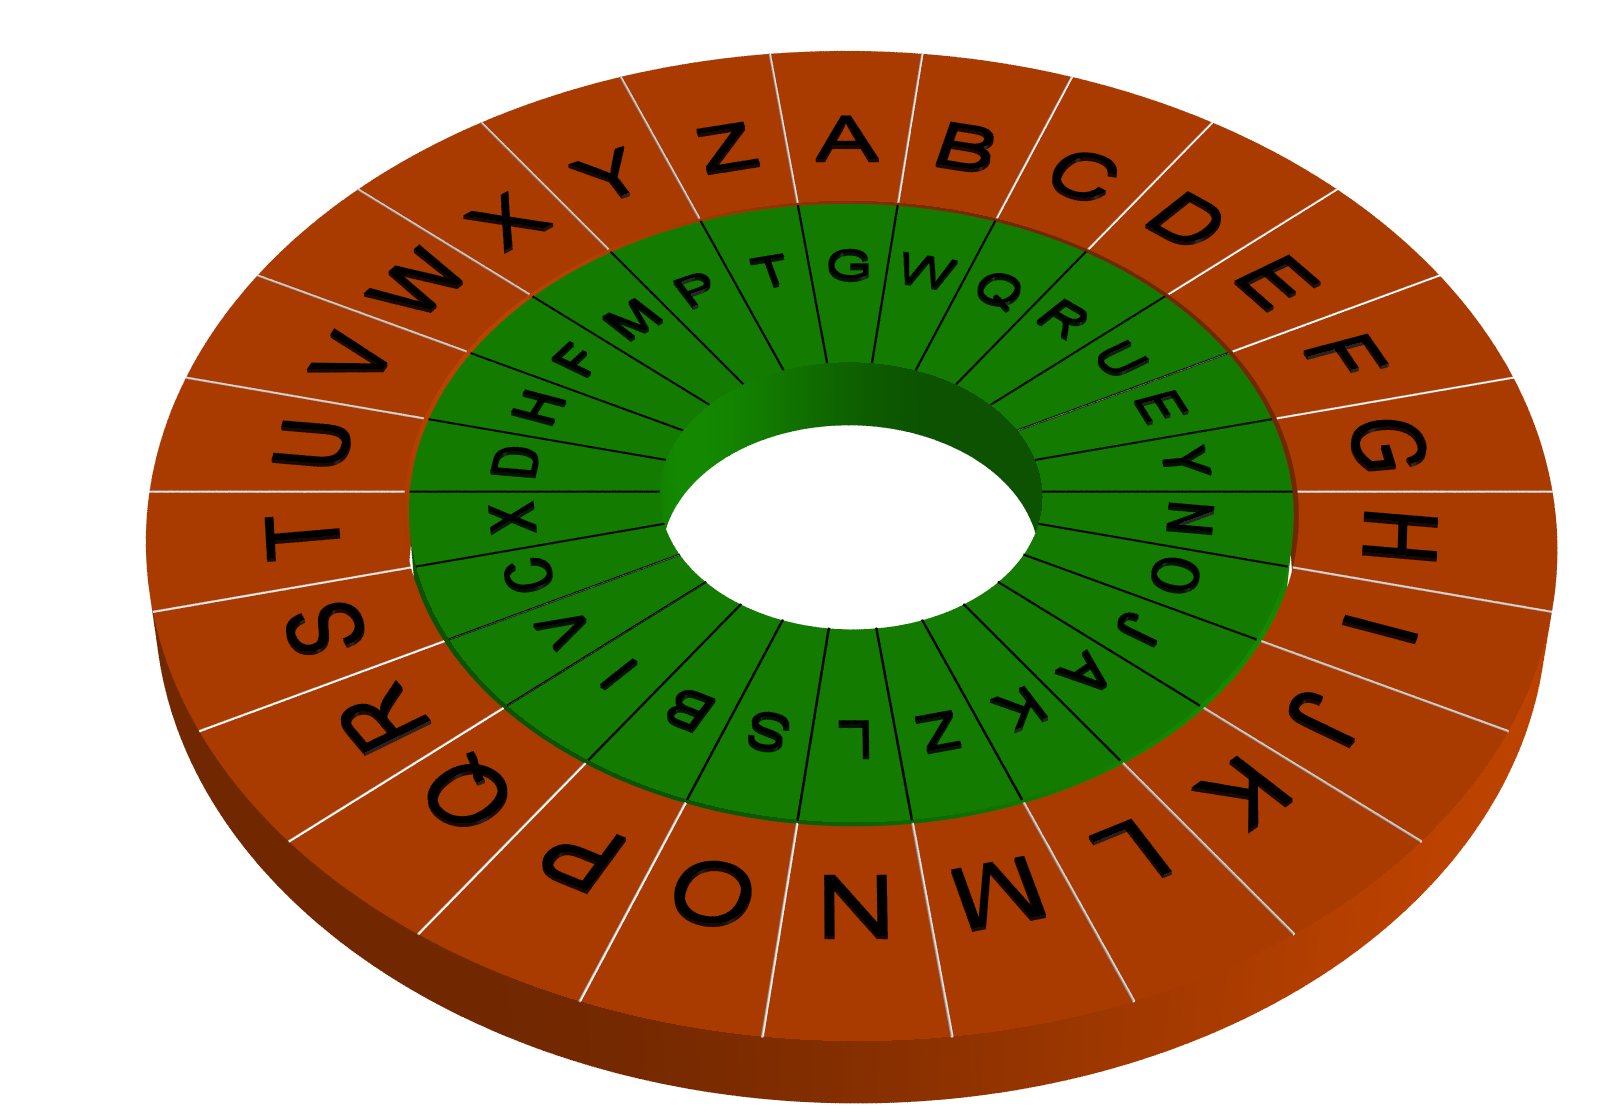
\includegraphics[width=0.4\textwidth]{figures/Enigma_0_bi_unesurune.png} 
 \qquad    
\uncover<4->{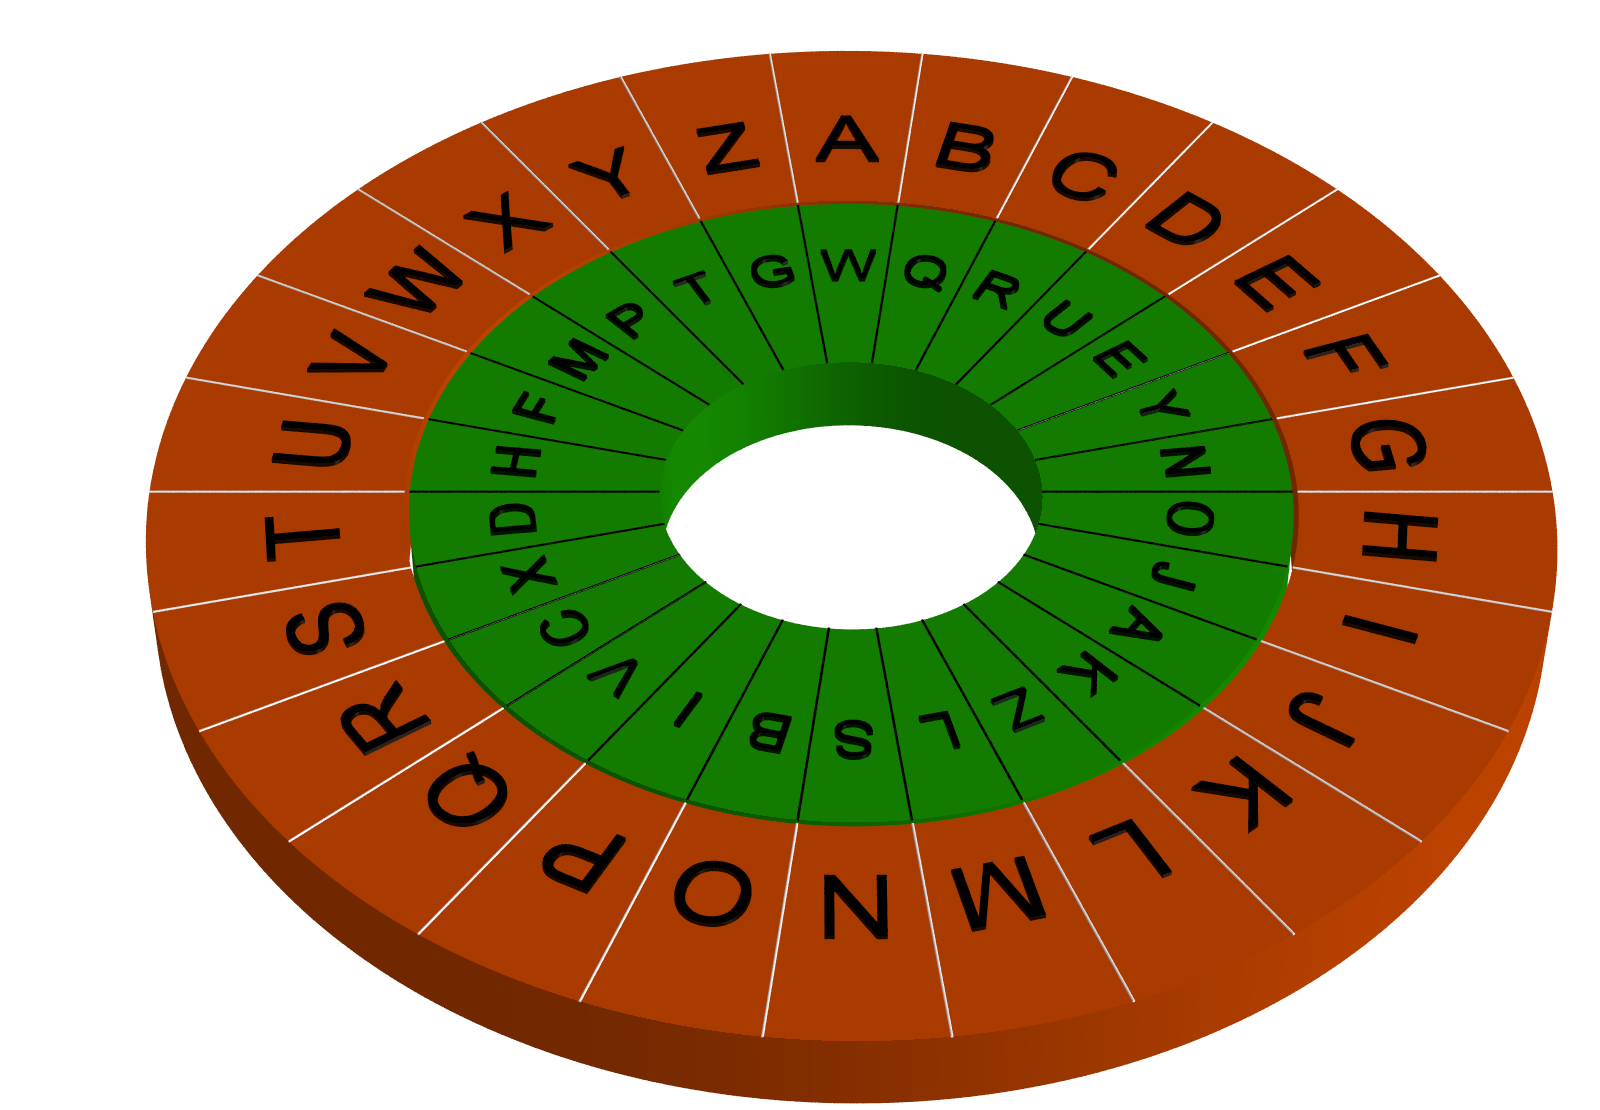
\includegraphics[width=0.4\textwidth]{figures/Enigma_1_bi_unesurune.png} }
}

\begin{enumerate}
  \item \textbf{Position initiale.} Le \prive{A} extérieur
  est en face du \public{G} intérieur (qui est la clé) et donc \prive{B} en face de \public{W}
\pause

  \item  \textbf{Première lettre.} L'opérateur tape  \prive{B} : la machine affiche \public{W}
\pause

  \item \textbf{Rotation.} L'anneau intérieur tourne de $1/26$ème de tour, 
  maintenant le \prive{A} extérieur est en face du \public{W}, le \prive{B} en face du \public{Q},...

%   \item \textbf{Deuxième lettre.} L'opérateur tape la deuxième lettre du message en clair \prive{A} : 
%   la machine affiche de nouveau \public{W}
%     
%   \item \textbf{Rotation.} L'anneau intérieur tourne de $1/26$ème de tour, maintenant le \prive{A} extérieur 
%   est en face du \public{Q}, le \prive{B} en face du \public{R}, le \prive{C} en face du \public{U},...
%   
%    \item \textbf{Troisième lettre.} L'opérateur tape la troisième lettre du message en clair \prive{C} : 
%    la machine affiche la correspondance \public{U} et effectue sa rotation.
%    
%    \item \textbf{Message codé.} Le message crypté est donc \public{WWU}
\end{enumerate}


\end{frame}

\begin{frame}
\evidence{Chiffrement du mot \prive{BAC} avec clé en position \prive{GWQR...}}

{\centering 
   \qquad         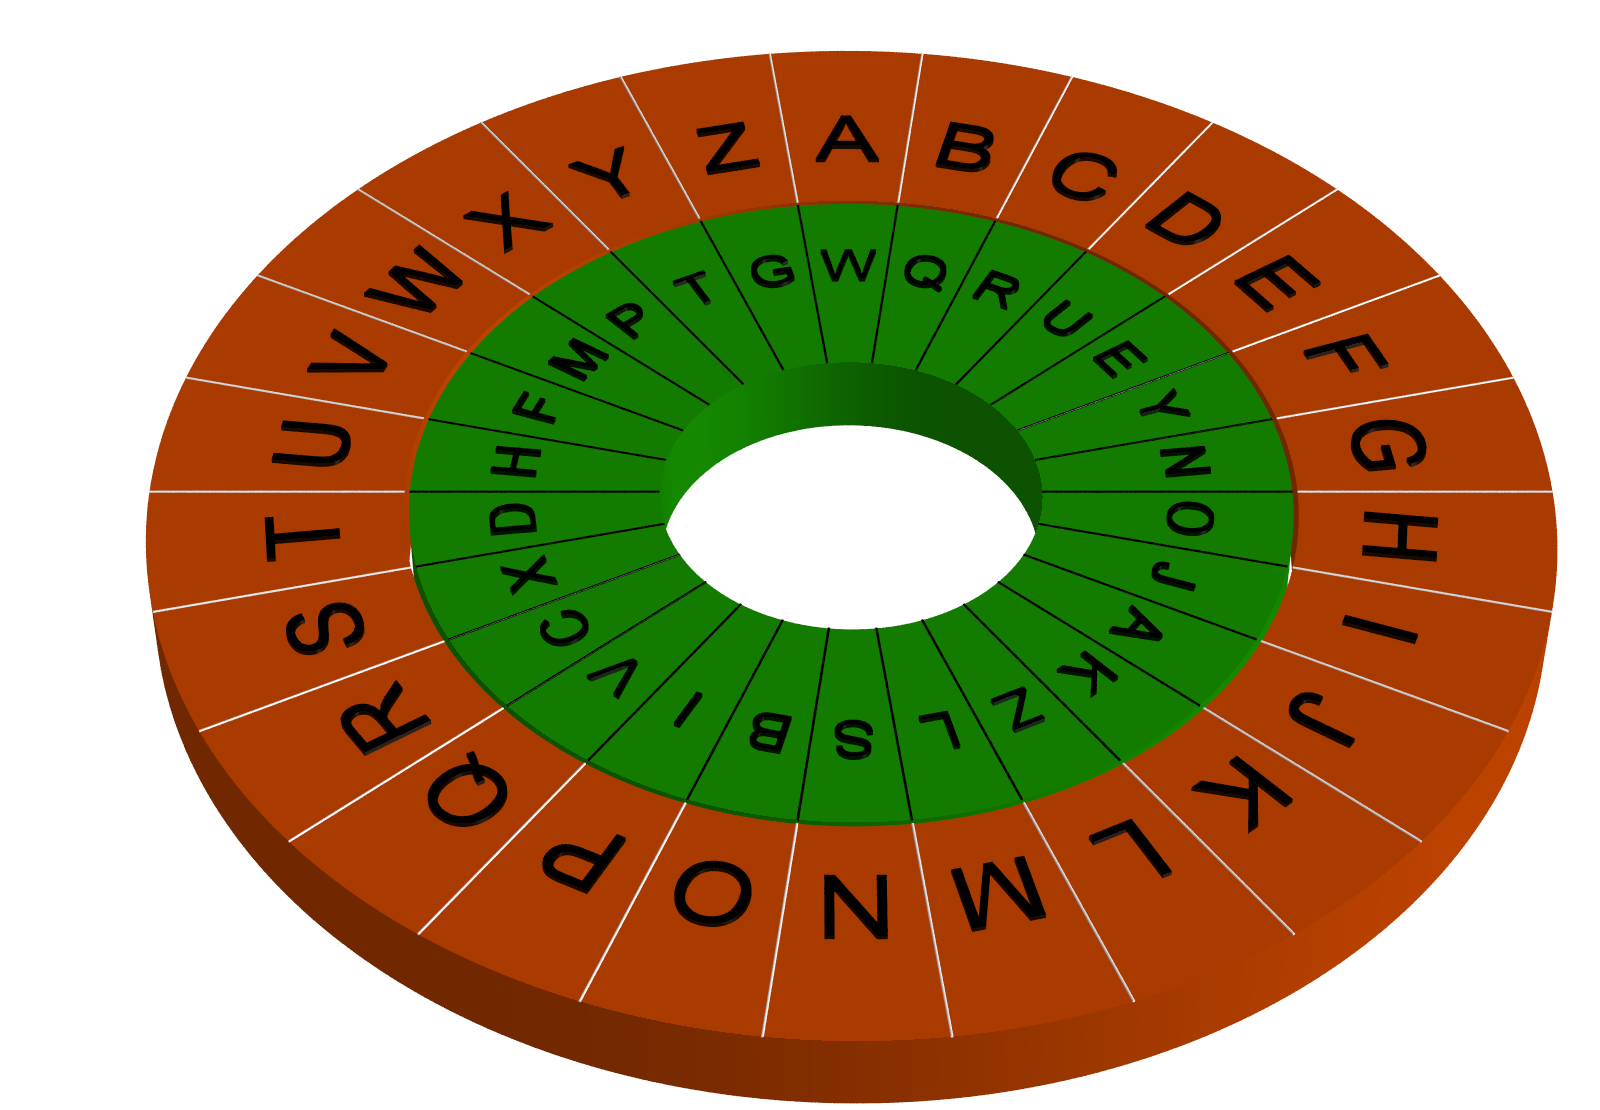
\includegraphics[width=0.4\textwidth]{figures/Enigma_1_bi_unesurune.png} 
 \qquad    
\uncover<3->{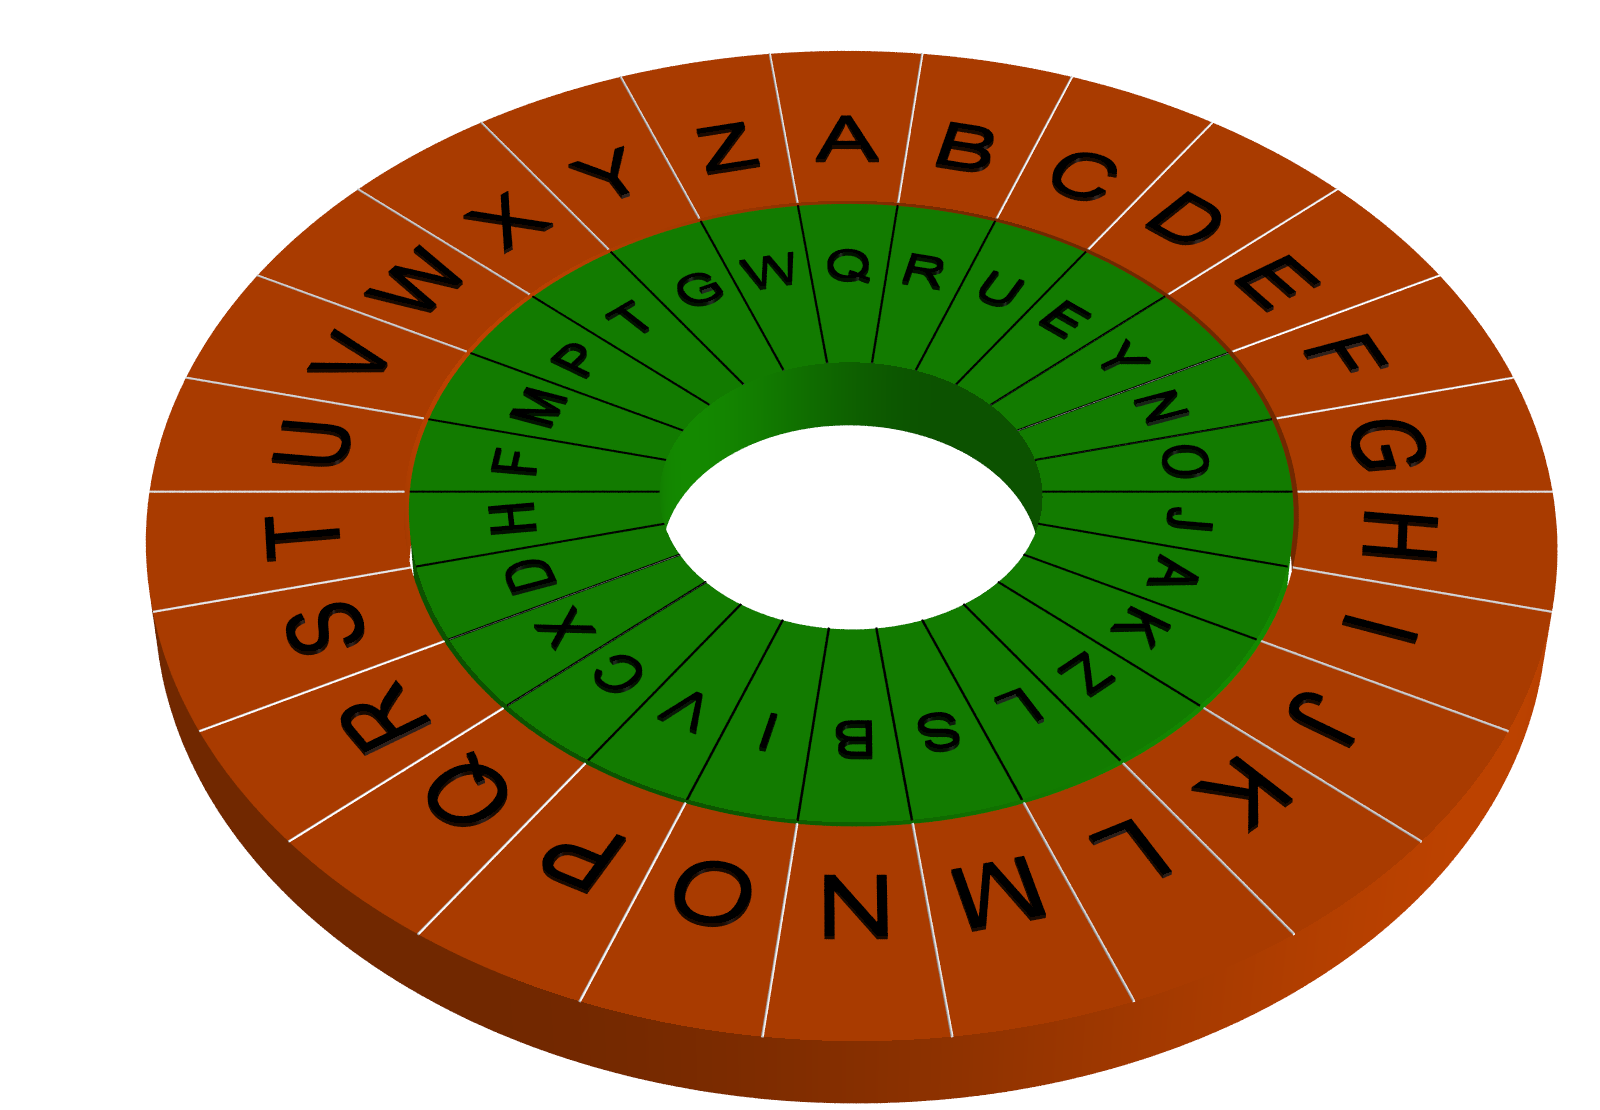
\includegraphics[width=0.4\textwidth]{figures/Enigma_2_bi_unesurune.png} }
}


\pause

\begin{enumerate}\setcounter{enumi}{3}
%   \item \textbf{Position initiale.} Le \prive{A} extérieur
%   est en face du \public{G} intérieur (qui est la clé) et donc \prive{B} en face de \public{W}
%   
%   \item  \textbf{Première lettre.} L'opérateur tape  \prive{B} : la machine affiche \public{W}
%   
%   \item \textbf{Rotation.} L'anneau intérieur tourne de $1/26$ème de tour, 
%   maintenant le \prive{A} extérieur est en face du \public{W}, le \prive{B} en face du \public{Q},...

  \item \textbf{Deuxième lettre.} L'opérateur tape \prive{A} : 
  la machine affiche de nouveau \public{W}
\pause

  \item \textbf{Rotation.} L'anneau intérieur tourne de $1/26$ème de tour, maintenant le \prive{A} extérieur 
  est en face du \public{Q}, le \prive{B} en face du \public{R}, le \prive{C} en face du \public{U},...
\pause

   \item \textbf{Troisième lettre.} Lettre tapée  \prive{C} : 
   la machine affiche \public{U} et effectue sa rotation
\pause

   \item \textbf{Message crypté.} Le message crypté est donc \public{WWU}
\end{enumerate}

\end{frame}



\begin{frame}
\evidence{Chiffrement du mot \prive{BAC}}


{\centering 
            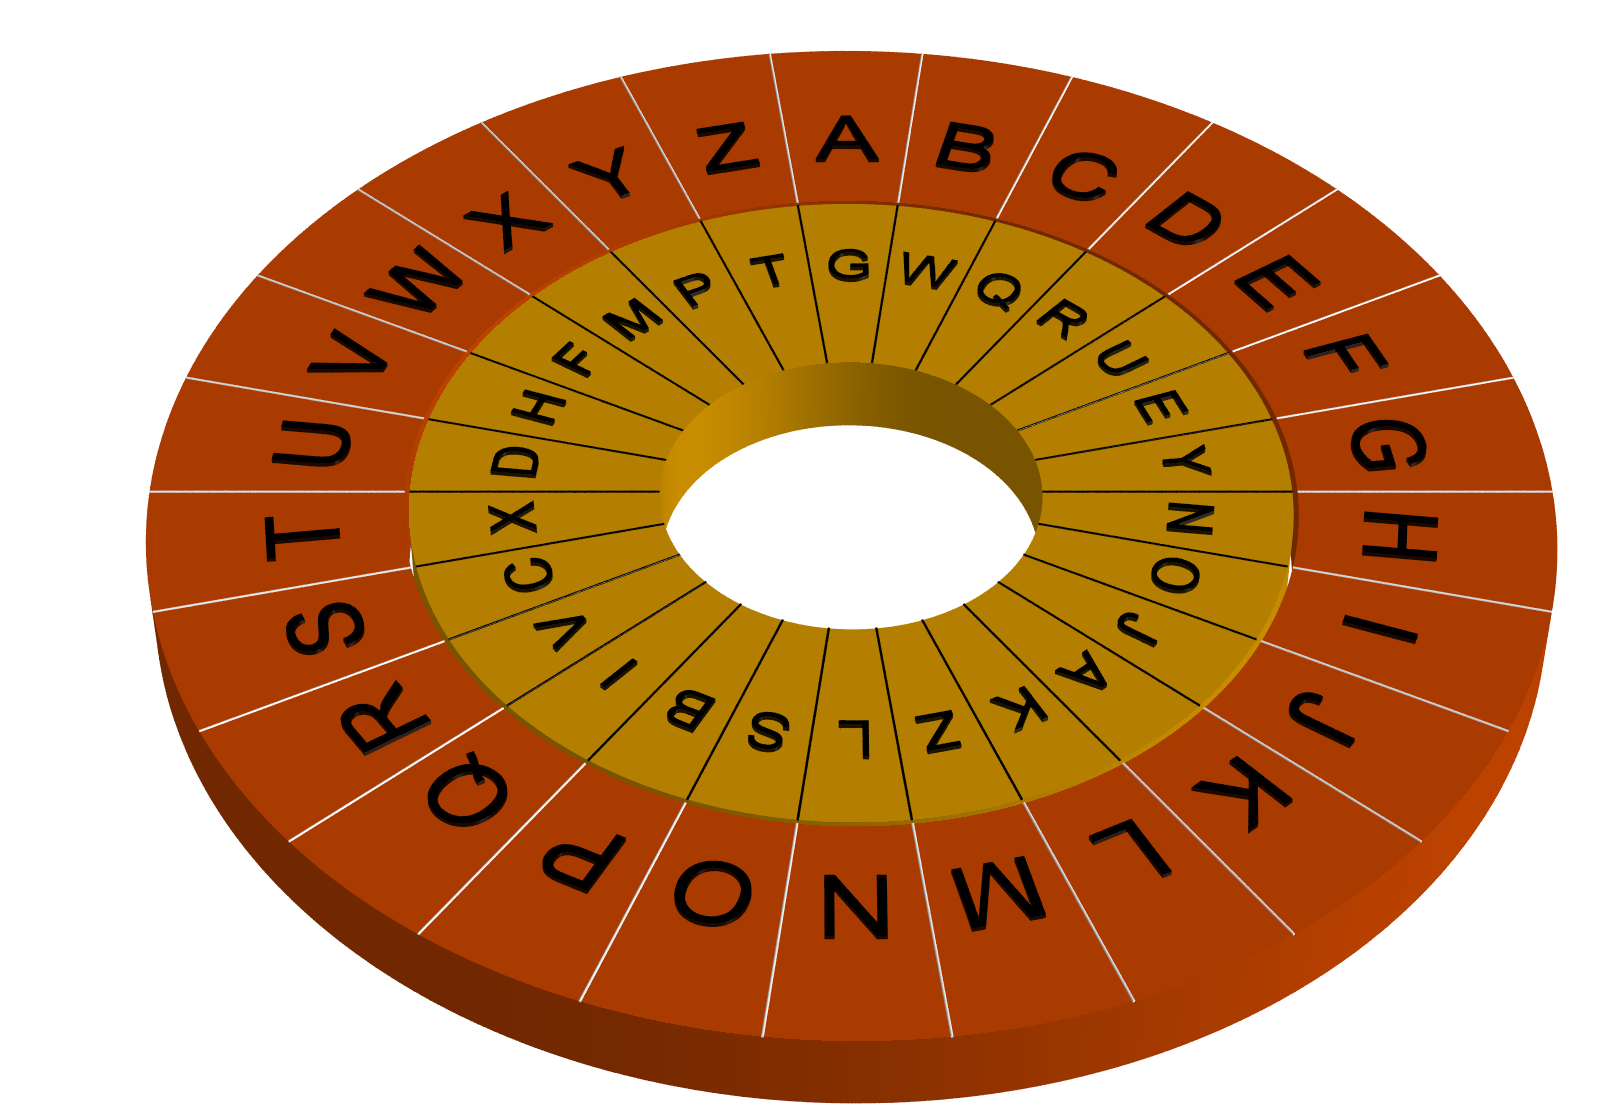
\includegraphics[width=0.4\textwidth]{figures/Enigma_0_bi_unesurdeux.png} 
            \qquad 
            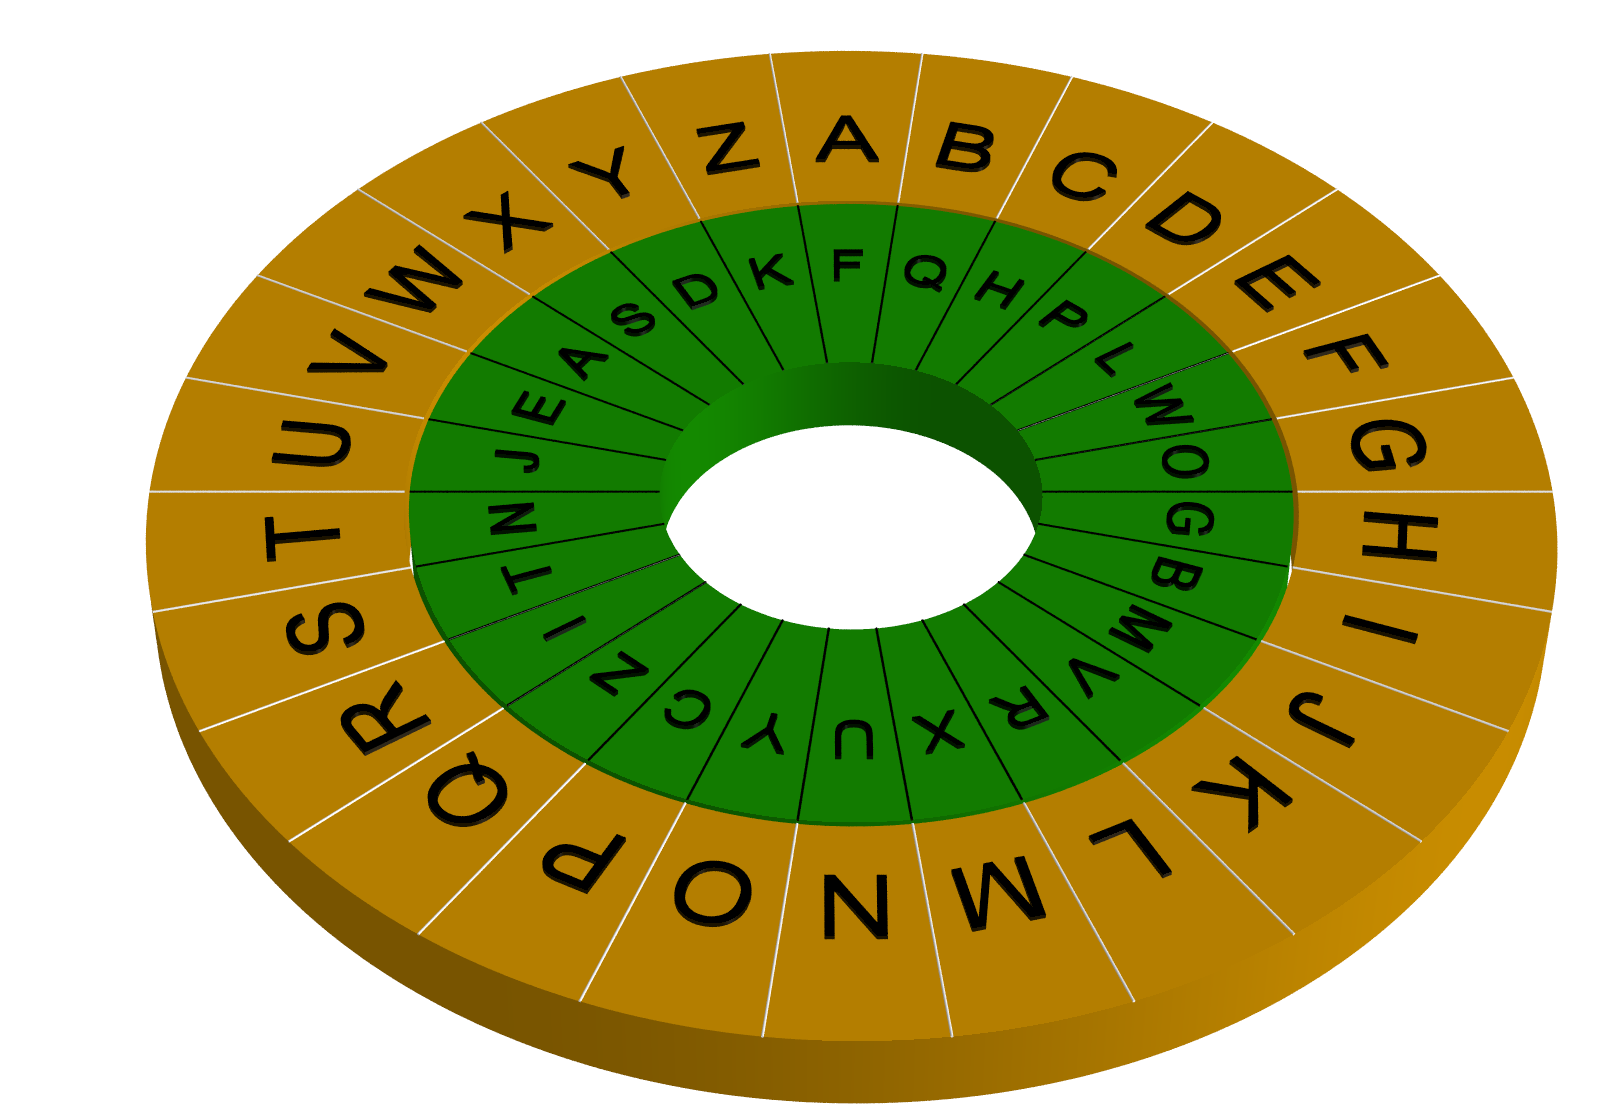
\includegraphics[width=0.4\textwidth]{figures/Enigma_0_tri_deuxsurdeux.png} 

}


\pause

\begin{enumerate}%\setcounter{enumi}{3}
%   \item \textbf{Position initiale.} Le \prive{A} extérieur
%   est en face du \public{G} intérieur (qui est la clé) et donc \prive{B} en face de \public{W}
%   
%   \item  \textbf{Première lettre.} L'opérateur tape  \prive{B} : la machine affiche \public{W}
%   
%   \item \textbf{Rotation.} L'anneau intérieur tourne de $1/26$ème de tour, 
%   maintenant le \prive{A} extérieur est en face du \public{W}, le \prive{B} en face du \public{Q},...

  \item \textbf{Première lettre.} L'opérateur tape \prive{B} : 
  la machine affiche \public{A}
\pause

  \item \textbf{Rotation(s).}... 
\end{enumerate}

\end{frame}
% 
% %%%%%%%%%%%%%%%%%%%%%%%%%%%%%%%%%%%%%%%%%%%%%%%%%%%%%%%%%%%%%%%%
% \section{Des zéros et des uns}
% 
% \begin{frame}
% 
% \begin{itemize}
%   \item Les deux seuls nombres sont $0$ et $1$
% \pause
% 
%   \item L'addition est celle de $\Zz/2\Zz$ :
% $$0+0=0 \qquad 0+1=1 \qquad 1+0=1 \qquad \color{red}{1+1=0}$$
% \pause
% 
%   \item
%   \begin{itemize}
%     \item Deux mots $m$ et $c$ composés de $0$ et de $1$
%     \pause
%     \item $m \oplus c$ addition \emph{bit} par \emph{bit}
%     \pause
%     \item Exemple $m = 10101010$, $c = 01110011$, notons $x= m \oplus c$ :
% \pause    
% $$\begin{array}{lccccccccc}
% m \quad &        & 1&0&1&0&1&0&1&0 \\
% c & \oplus & 0&1&1&1&0&0&1&1 \\
% \hline
% \pause
% x &        & 1&1&0&1&1&0&0&1 \\
% \end{array}$$
%   \end{itemize}
%   
%  \pause 
%   \item $m$ est le message en clair, $c$ la clé de cryptage et $x$ le message crypté
%  
% \pause 
%   \item Comment déchiffrer le message ?
%   \pause
%   \begin{itemize}
%     \item $0+0=0$ et $1+1=0$  alors $-1=+1$
%     \pause
%     \item $x\oplus c = m$
%     \pause
%     \item Preuve : $x \oplus c = (m \oplus c) \oplus c = m \oplus (c \oplus c) = m \oplus 0 = m$
%   \end{itemize}
% \end{itemize}
% 
% \end{frame}



%%%%%%%%%%%%%%%%%%%%%%%%%%%%%%%%%%%%%%%%%%%%%%%%%%%%%%%%%%%%%%%%
\section{La ronde des chiffres : DES}

\begin{frame}

\begin{itemize}
  \item Enigma change mécaniquement d'alphabet
\pause  
  \item Méthode numérique : le DES  : \emph{Data Encryption Standard}
\pause  
  \item But : générer une clé aléatoire de grande longueur
\pause 
  \item Génération pseudo-aléatoire
\end{itemize}

\pause 

\begin{exemple}
\begin{itemize}
  \item Soit $(u_n)$  définie par $(a,b)$ et $u_0$ et 
$$u_{n+1} \equiv a\times u_n + b \pmod{26}$$
\vspace*{-4ex}
\pause  
  \item Exemple : $a=2$, $b=5$ et $u_0=6$ \\
\pause  
{\small $6 \quad 17\quad 13\quad 5\quad 15 \quad9\quad 23\quad 25\quad 3 \quad11\quad 1 \quad7\quad 19\quad 17\quad 13\quad 5 \ldots$}
\pause  
  \item $(a,b,u_0)$  la \defi{clé principale}
\pause  
  \item $(u_n)_{n\in\Nn}$ les \defi{clés secondaires}
\end{itemize}
  
\end{exemple}
\end{frame}


\begin{frame}

\evidence{DES simplifié}
\pause  

\begin{itemize} 
  \item Les additions se font \emph{terme} à \emph{terme}
\pause    
  \item Modulo $10$  
\pause    
          $$[1 \ 2 \ 3 \  4] \oplus [7\  8\  9\  0] = [8\  0\  2\  4]$$
\pause    
  \item Le message est découpé en blocs de longueur $8$ 
\pause   
  \item La clé est de longueur $4$
\pause    
\begin{itemize}
  \item Message $M = [1\  2\  3\  4\  5\  6\  7\  8]$ 
\pause    
  \item Clé $C=[3\  1\  3\  2]$
\end{itemize}
\end{itemize}

\end{frame}


\begin{frame}


\evidence{\'Etape 1. Premier tour}
$$M_0 = [ G_0 \ \|\  D_0] = [1\  2\  3\  4\  \| \ 5\  6\  7\  8]$$
\pause

$$M_1 = [ D_0 \ \|\  C \oplus \sigma(G_0)]$$
\pause

\begin{enumerate}
  \item On échange la partie droite et la partie gauche de $M_0$ 
\pause  
$$M_0  \longmapsto  [5\  6\  7\  8\  \|\  1\  2\  3\  4]$$
\pause
  \item Sur la nouvelle partie droite, on permute circulairement les nombres
\pause  
$$\longmapsto  [5\  6\  7\  8\  \|\ 2\  3\  4\  1]$$
\pause

  \item Puis on ajoute la clé secrète $C$ à droite (ici $C=[3\  1\  3\  2]$)
\pause  
$$\longmapsto  [5\  6\  7\  8\  \| \ 5\  4\  7\  3] = M_1$$
\end{enumerate}

\end{frame}


\begin{frame}


\evidence{Tours suivants}
$$\text{Si} \quad M_i=[G_i \ \| \ D_i] \quad \text{alors} \quad M_{i+1} = [ D_i \ \| \ C \oplus \sigma(G_i)]$$

\pause

\evidence{\'Etape 2. Deuxième tour}
$$M_1 = [5\  6\  7\  8\  \|\ 5\  4\  7\  3]$$
\pause
\begin{enumerate}
  \item On échange la partie droite et la partie gauche de $M_1$
$$M_1  \longmapsto  [5\  4\  7\  3\  \| \ 5\  6\  7\  8]$$
\pause
  \item Sur la nouvelle partie droite, on applique $\sigma$
$$\longmapsto  [5\  4\  7\  3\  \| \ 6\  7\  8\  5]$$
\pause
  \item Puis on ajoute la clé secrète $C$ à droite
$$\longmapsto  [5\  4\  7\  3\  \| \ 9\  8\  1\  7] = M_2$$
\end{enumerate}
\pause
$$X=M_2 = [5\  4\  7\  3\ 9\  8\  1\  7]$$

\end{frame}


\end{document}
